\chapter{Technical Background}
\label{chp:techbackground}

We now present some technical background that will be required to understand the remaining of this dissertation.

\section{Trajectory and data information}
\label{sec:tech_data}

Spatio-temporal datasets usually come in the form of a set of tuples $\{O_{id}, \phi, \lambda, t\}$. Where: $O_{id}$
uniquely identifies a \ac{mo}; $t$ corresponds to the timestamp that the \ac{gps} position was extracted; $\phi$ and
$\lambda$ correspond to the latitude and longitude of the \ac{mo} respectively, at a given timestamp $t$. Each \ac{mo}
represented by a $O_{id}$ has a trajectory $T_{id}$ associated with it, being a trajectory defined as follows.

\begin{Def}
Given an $O_{id}$, an trajectory $T_{id}$ consists of a sequence of 3-D points, belonging to $O_{id}$ in the form of
$<(\phi_0, \lambda_0, t_0), (\phi_1, \lambda_1, t_1), ..., (\phi_n, \lambda_n, t_n)>$, with $n \in \mathbb{N}$ and $t_0
< t_1 < ... < t_n$.
\end{Def}

\begin{table}[h!]
    \centering
    \caption{Conversion from \ac{wgs84} to $\mathbb{R}^2$}
    \label{tbl:coordinates}
    \begin{tabular}{c | c | c | c }
        \toprule
        \multicolumn{2}{ c | }{\textbf{\ac{wgs84}}} &
        \multicolumn{2}{ c }{$\mathbb{R}^2$}\\
        \toprule
        \textbf{$\phi$} & \textbf{$\lambda$} & \textbf{$x$} & \textbf{$y$} \\
        \toprule
        $0^\circ$         & $0^\circ$         & 0          & 0 \\
        $38.018470^\circ$ & $23.845089^\circ$ & 2654452.0  & 4203597.2 \\
        $39.9048^\circ$   & $116.368^\circ$   & 12954167.2 & 4412163.5 \\
        $40.0623^\circ$   & $116.582^\circ$   & 12977989.8 & 4429577.9 \\
        $40.0114^\circ$   & $116.551^\circ$   & 12974538.9 & 4423950.0 \\
        $52.5863^\circ$   & $13.2363^\circ$   & 1473474.2  & 5814321.9 \\
        \bottomrule
    \end{tabular}
\end{table}

\ac{gps} coordinates are often represented using the \ac{wgs84} \citep{wgs84}, which can make some mathematical
operations needed by the algorithm proposed in this dissertation (e.g. vectorial operations) harder to be performed.
Given that limitation, once the coordinates are read from a dataset, transformations from \ac{wgs84} to the
$\mathbb{R}^2$ system are made. We use $0^\circ$ as both latitude and longitude coordinates for our origin point in the
$\mathbb{R}^2$ system and execute the algorithm used by the \ac{whoi} to perform the conversion from \ac{wgs84} to
$\mathbb{R}^2$ on the fly \citep{latlogtoxy}. Please refer to \tabref{tbl:coordinates} for some examples of \ac{wgs84}
coordinates being translated to $\mathbb{R}^2$, using the algorithm provided by \ac{whoi}.

It is worth noting that real world datasets do not guarantee that all points of all trajectories are sampled in the same
rate. In a ideal world, a perfect spatio-temporal dataset would have entries as described in \tabref{tbl:ideal_rate},
where one can see that each $O_{id}$ has its position sampled in intervals of 1 $t$ unit. However,
\tabref{tbl:real_rate}presents how \acp{mo} in real-world datasets have their position sampled over time: no fixed rate
interval due to transmission noises, precision issues and other problems that can make the sample rate varying a lot
from one $O_{id}$ to another. Therefore, we need to have a way to be able to compare and group points belonging to the
same logical time interval. With that in mind, we divided the time extent in buckets of size $\sigma$, where $\sigma$
should be chosen accordingly to the dataset being analyzed, based on the sampling rate of points. Hence, from this point
forward, every time when we refer to any timestamp $t_i$ we are actually talking about the $i_{th}$ time bucket (or time
slot) of size $\sigma$.

\begin{table}
    \centering
    \begin{minipage}{0.5\textwidth}
        \centering
        \caption{Ideal dataset sample rate}
        \label{tbl:ideal_rate}
        \begin{tabular}{c c c c}
            \toprule
            \textbf{$O_{id}$} & \textbf{$\phi$} & \textbf{$\lambda$} & \textbf{$t$} \\
            \toprule
            0 & 38.018470 & 23.845089 & 0 \\
            1 & 38.018069 & 23.845179 & 0 \\
            2 & 38.018241 & 23.845530 & 0 \\
            3 & 38.017440 & 23.845499 & 0 \\
            4 & 38.015609 & 23.844780 & 0 \\
            \bottomrule
            0 & 38.015609 & 23.844780 & 1 \\
            1 & 38.014018 & 23.844780 & 1 \\
            2 & 38.012569 & 23.844869 & 1 \\
            3 & 38.011600 & 23.845360 & 1 \\
            4 & 38.010650 & 23.845550 & 1 \\
            \bottomrule
            0 & 38.010478 & 23.845100 & 2 \\
            1 & 38.010478 & 23.845100 & 2 \\
            2 & 38.010508 & 23.844640 & 2 \\
            3 & 38.010520 & 23.844530 & 2 \\
            4 & 38.010520 & 23.844530 & 2 \\
            \bottomrule
        \end{tabular}
    \end{minipage}%
    \hfill
    \begin{minipage}{0.5\textwidth}
        \centering
        \caption{Real-world dataset sample rate}
        \label{tbl:real_rate}
        \begin{tabular}{c c c c}
            \toprule
            \textbf{$O_{id}$} & \textbf{$\phi$} & \textbf{$\lambda$} & \textbf{$t$} \\
            \toprule
            0 & 38.018470 & 23.845089 & 4 \\
            1 & 38.018069 & 23.845179 & 0 \\
            2 & 38.018241 & 23.845530 & 1 \\
            3 & 38.017440 & 23.845499 & 10 \\
            4 & 38.015609 & 23.844780 & 8 \\
            \bottomrule
            0 & 38.015609 & 23.844780 & 6 \\
            1 & 38.014018 & 23.844780 & 5 \\
            2 & 38.012569 & 23.844869 & 2 \\
            3 & 38.011600 & 23.845360 & 16 \\
            4 & 38.010650 & 23.845550 & 12 \\
            \bottomrule
            0 & 38.010478 & 23.845100 & 14 \\
            1 & 38.010478 & 23.845100 & 6 \\
            2 & 38.010508 & 23.844640 & 3 \\
            3 & 38.010520 & 23.844530 & 25 \\
            4 & 38.010520 & 23.844530 & 30 \\
            \bottomrule
        \end{tabular}
    \end{minipage}
\end{table}

\begin{table}[h!]
    \centering
    \caption{Mapping points from \tabref{tbl:real_rate} to its correspondent time slot, using $\sigma = 3$}
    \label{tbl:timeslot}
    \begin{tabular}{c c c c c}
        \toprule
        \textbf{$O_{id}$} & \textbf{$\phi$} & \textbf{$\lambda$} & \textbf{$t$} & \textbf{Time slot} \\
        \toprule
        0 & 38.018470 & 23.845089 & 4 & 1 \\
        1 & 38.018069 & 23.845179 & 0 & 0 \\
        2 & 38.018241 & 23.845530 & 1 & 0 \\
        3 & 38.017440 & 23.845499 & 10 & 3 \\
        4 & 38.015609 & 23.844780 & 8  & 2 \\
        \bottomrule
        0 & 38.015609 & 23.844780 & 6 & 2 \\
        1 & 38.014018 & 23.844780 & 5 & 1 \\
        2 & 38.012569 & 23.844869 & 2 & 0 \\
        3 & 38.011600 & 23.845360 & 16 & 5 \\
        4 & 38.010650 & 23.845550 & 12 & 4 \\
        \bottomrule
        0 & 38.010478 & 23.845100 & 14 & 4 \\
        1 & 38.010478 & 23.845100 & 6 & 2 \\
        2 & 38.010508 & 23.844640 & 3 & 1 \\
        3 & 38.010520 & 23.844530 & 25 & 8 \\
        4 & 38.010520 & 23.844530 & 30 & 10 \\
        \bottomrule
    \end{tabular}
\end{table}

After dividing the time extent of the dataset presented by \tabref{tbl:real_rate} using $\sigma = 3$,
\tabref{tbl:timeslot} shows in which time slot each $O_{id}$ entry will end up at. The assignment of the time slot is
made by dividing the timestamp value by the bucket size $\sigma$ and then performing a floor operation, as shown in
\eqnref{eq:timeslot}.

\begin{equation}
    \label{eq:timeslot}
    s = \floor*{\frac{t}{\sigma}}
\end{equation}

\section{Flock pattern}
\label{sec:tech_flock}
We use the same definition of flock from Vieira et al. \citep{vieira}:

\begin{Def}
\label{def:flock}
Given a set of trajectories $\mathcal{T}$, a minimum number of trajectories $\mu > 1$ ($\mu \in \mathbb{N}$), a maximum
distance $\epsilon > 0$ defined over the distance function $d$, and a minimum time duration $\delta > 1$ ($\delta \in
\mathbb{N}$). A flock pattern $Flock (\mu, \epsilon, \delta)$ reports all maximal size collections $\mathcal{F}$ of
trajectories where: for each $f_k$ in $\mathcal{F}$, the number of trajectories in $f_k$ is greater or equal than $\mu$
($|f_k| \ge \mu$) and there exist $\delta$ consecutive timestamps such that for every $t_i \in [f_k^{t_1}...f_k^{t_1 +
\delta}]$, there is a disk with center $c_k^{t_i}$ and radius $\epsilon/2$ covering all points in $f_k^{t_i}$. That is:
$\forall f_k \in \mathcal{F}, \forall t_i \in [f_k^{t_1}...f_k^{t_1 + \delta}], \forall T_j \in f_k: |f_k | \ge \mu,
d(p_j^{t_i},c_k^{t_i}) \le \epsilon/2$.
\end{Def}

\begin{figure}[h!]
    \centering
    \caption{T1, T2 and T3 form a flock of size $\mu =3$ with minimum length of $\delta = 3$ time slots and with a disk
        diameter of size $\epsilon = d$}
    \centerline{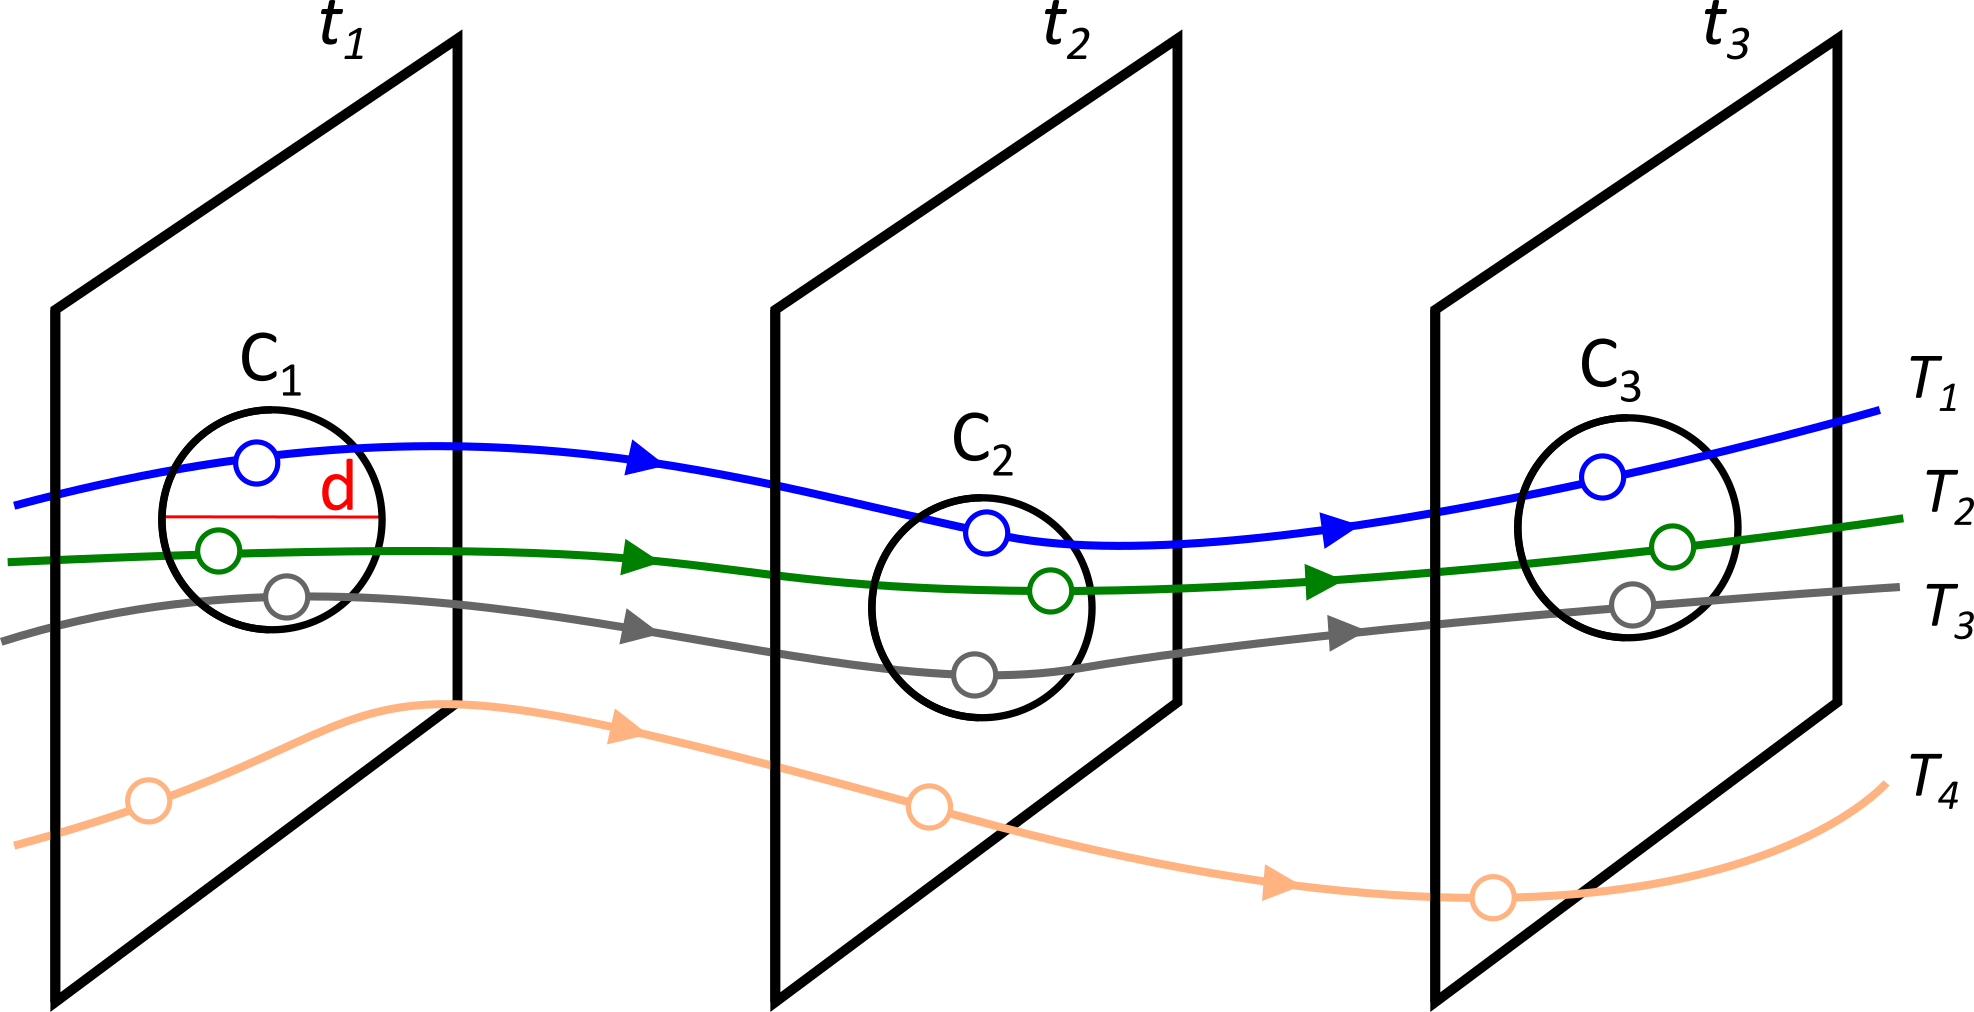
\includegraphics[width=\textwidth]{images/flock_2.png}}
    \footnotesize{Source: Made by the author.}
    \label{fig:flock2}
\end{figure}

In other words, what \defref{def:flock} states is that a flock pattern basically consists in a set of at least $\mu$
trajectories (where each trajectory $T_{id}$ belongs to the \ac{mo} represented by $O_{id}$) that stay together for a
minimum time extent $\delta$.  Additionally, in order to be considered a flock, there must exist a disk, with radius
$\epsilon/2$, that encloses all points of all trajectories for each time slot. Hence, we have a flock pattern relying on
three key parameters:

\begin{enumerate}
    \item $\mu$: the minimum number of trajectories, in order to be considered a flock
    \item $\epsilon$: diameter of the disk that needs to enclose the trajectories for each time slot
    \item $\delta$: the minimum number of time slot units that the trajectories need to stay together
\end{enumerate}

This definition is well depicted in \figref{fig:flock2}, where you can see for each time slot $t_i$ it exists a disk of
diameter $\epsilon = d$ enclosing the points of trajectories $T_1$, $T_2$ and $T_3$. Thus, if we have set our flock
parameters to $\mu = 3$, $\epsilon = d$ and $\delta = 3$, we would have found the flock pattern $f = \{T_1, T_2, T_3\}$
shown in \figref{fig:flock2}. It is worth noting that trajectory $T_4$ could not be part of the flock pattern because it
was not possible to find a disk of diameter $d$ that would enclose 2 more trajectories with $T_4$ in each time slot
$t_i$.

\subsection{Disk discovery}
\label{subsec:disk_discovery}

One of the most important part that enables the flock pattern identification is how to efficiently discover the disks
that can enclose potential flock patterns. Since the disk does not need to have its center matching any of the points in
the dataset, there can be infinite places to look for disk in the dataset space. Vieira et al. \citep{vieira} proposed a
way to reduce that search space to a finite number of locations, which we will explain in the remaining of this section
and will be used in the algorithm proposed in this dissertation.

We can easily find two circles that intersect two points using some vectorial operations as shown in
Algorithm~\ref{alg:disks} below.

Given two \ac{gps} points $p_1$ and $p_2$, we get the values of $x1$ and $y1$, which will correspond to the longitude
and latitude in meters (such conversion is mentioned in \secref{sec:tech_data}) of $p_1$, and $x2$ and $y2$ being the
equivalent of $p_2$ (lines 1 to 4). We know that the centers of the two disks $c_1$ and $c_2$ that can be generated by
those two points, lie in the line that is orthogonal to points $p_1$ and $p_2$ and passes through the midpoint $p_m$ of
those same points. After calculating $p_m$ (lines 6 and 7) we convert those same points into a vector $v$ (lines 9 and
10) and calculate its length (line 12), which will be used later to normalize $v$. Line 13 calculates the distance $c_d$
that the centers are from $p_m$ whereas lines 15 and 16 calculate the orthogonal vector $o$ for $v$, which will guide
the direction for the disks centers. The algorithm ends by finding the center $c_1$ by adding $p_m$ to the product of
$o$ and $c_d$, and $c_2$ by subtracting $p_m$ from the product of $o$ and $c_d$. The disks that we could find are
depicted in \figref{fig:disks_discovery}.

\begin{algorithm}[h!]
\caption{Disks Discovery}
\label{alg:disks}
\begin{algorithmic}[1]
    \State $x1 \gets p1.longitudeMeters$
    \State $y1 \gets p1.latitudeMeters$
    \State $x2 \gets p2.longitudeMeters$
    \State $y2 \gets p2.latitudeMeters$
    \State
    \State $midX \gets \frac{x1 + x2}{2}$
    \State $midY \gets \frac{y1 + y2}{2}$
    \State
    \State $vectorX \gets x2 - x1$
    \State $vectorY \gets y2 - y1$
    \State
    \State $pointsDistance \gets \sqrt{vectorX^2 + vectorY^2}$
    \State $centerDistFromMidPoint \gets \sqrt{(\frac{\epsilon}{2})^2 - (\frac{pointsDistance}{2})^2}$
    \State
    \State $orthogonalVectorX \gets vectorY$
    \State $orthogonalVectorY \gets -vectorX$
    \State
    \State $normalizedOrtVectorX \gets \frac{orthogonalVectorX}{pointsDistance}$
    \State $normalizedOrtVectorY \gets \frac{orthogonalVectorY}{pointsDistance}$
    \State
    \State $c1X \gets midX + (centerDistFromMidPoint * normalizedOrtVectorX)$
    \State $c1Y \gets midY + (centerDistFromMidPoint * normalizedOrtVectorY)$
    \State
    \State $c2X \gets midX - (centerDistFromMidPoint * normalizedOrtVectorX)$
    \State $c2Y \gets midY - (centerDistFromMidPoint * normalizedOrtVectorY)$
\end{algorithmic}
\end{algorithm}

\begin{figure}[h!]
    \centering
    \caption{Two disks with radius $\epsilon/2$ that are found based on points $p_1$ and $p_2$. $c_1$ and $c_2$ stand
        for the disks centers and $m$ represents the midpoint between $p_1$ and $p_2$.}
    \centerline{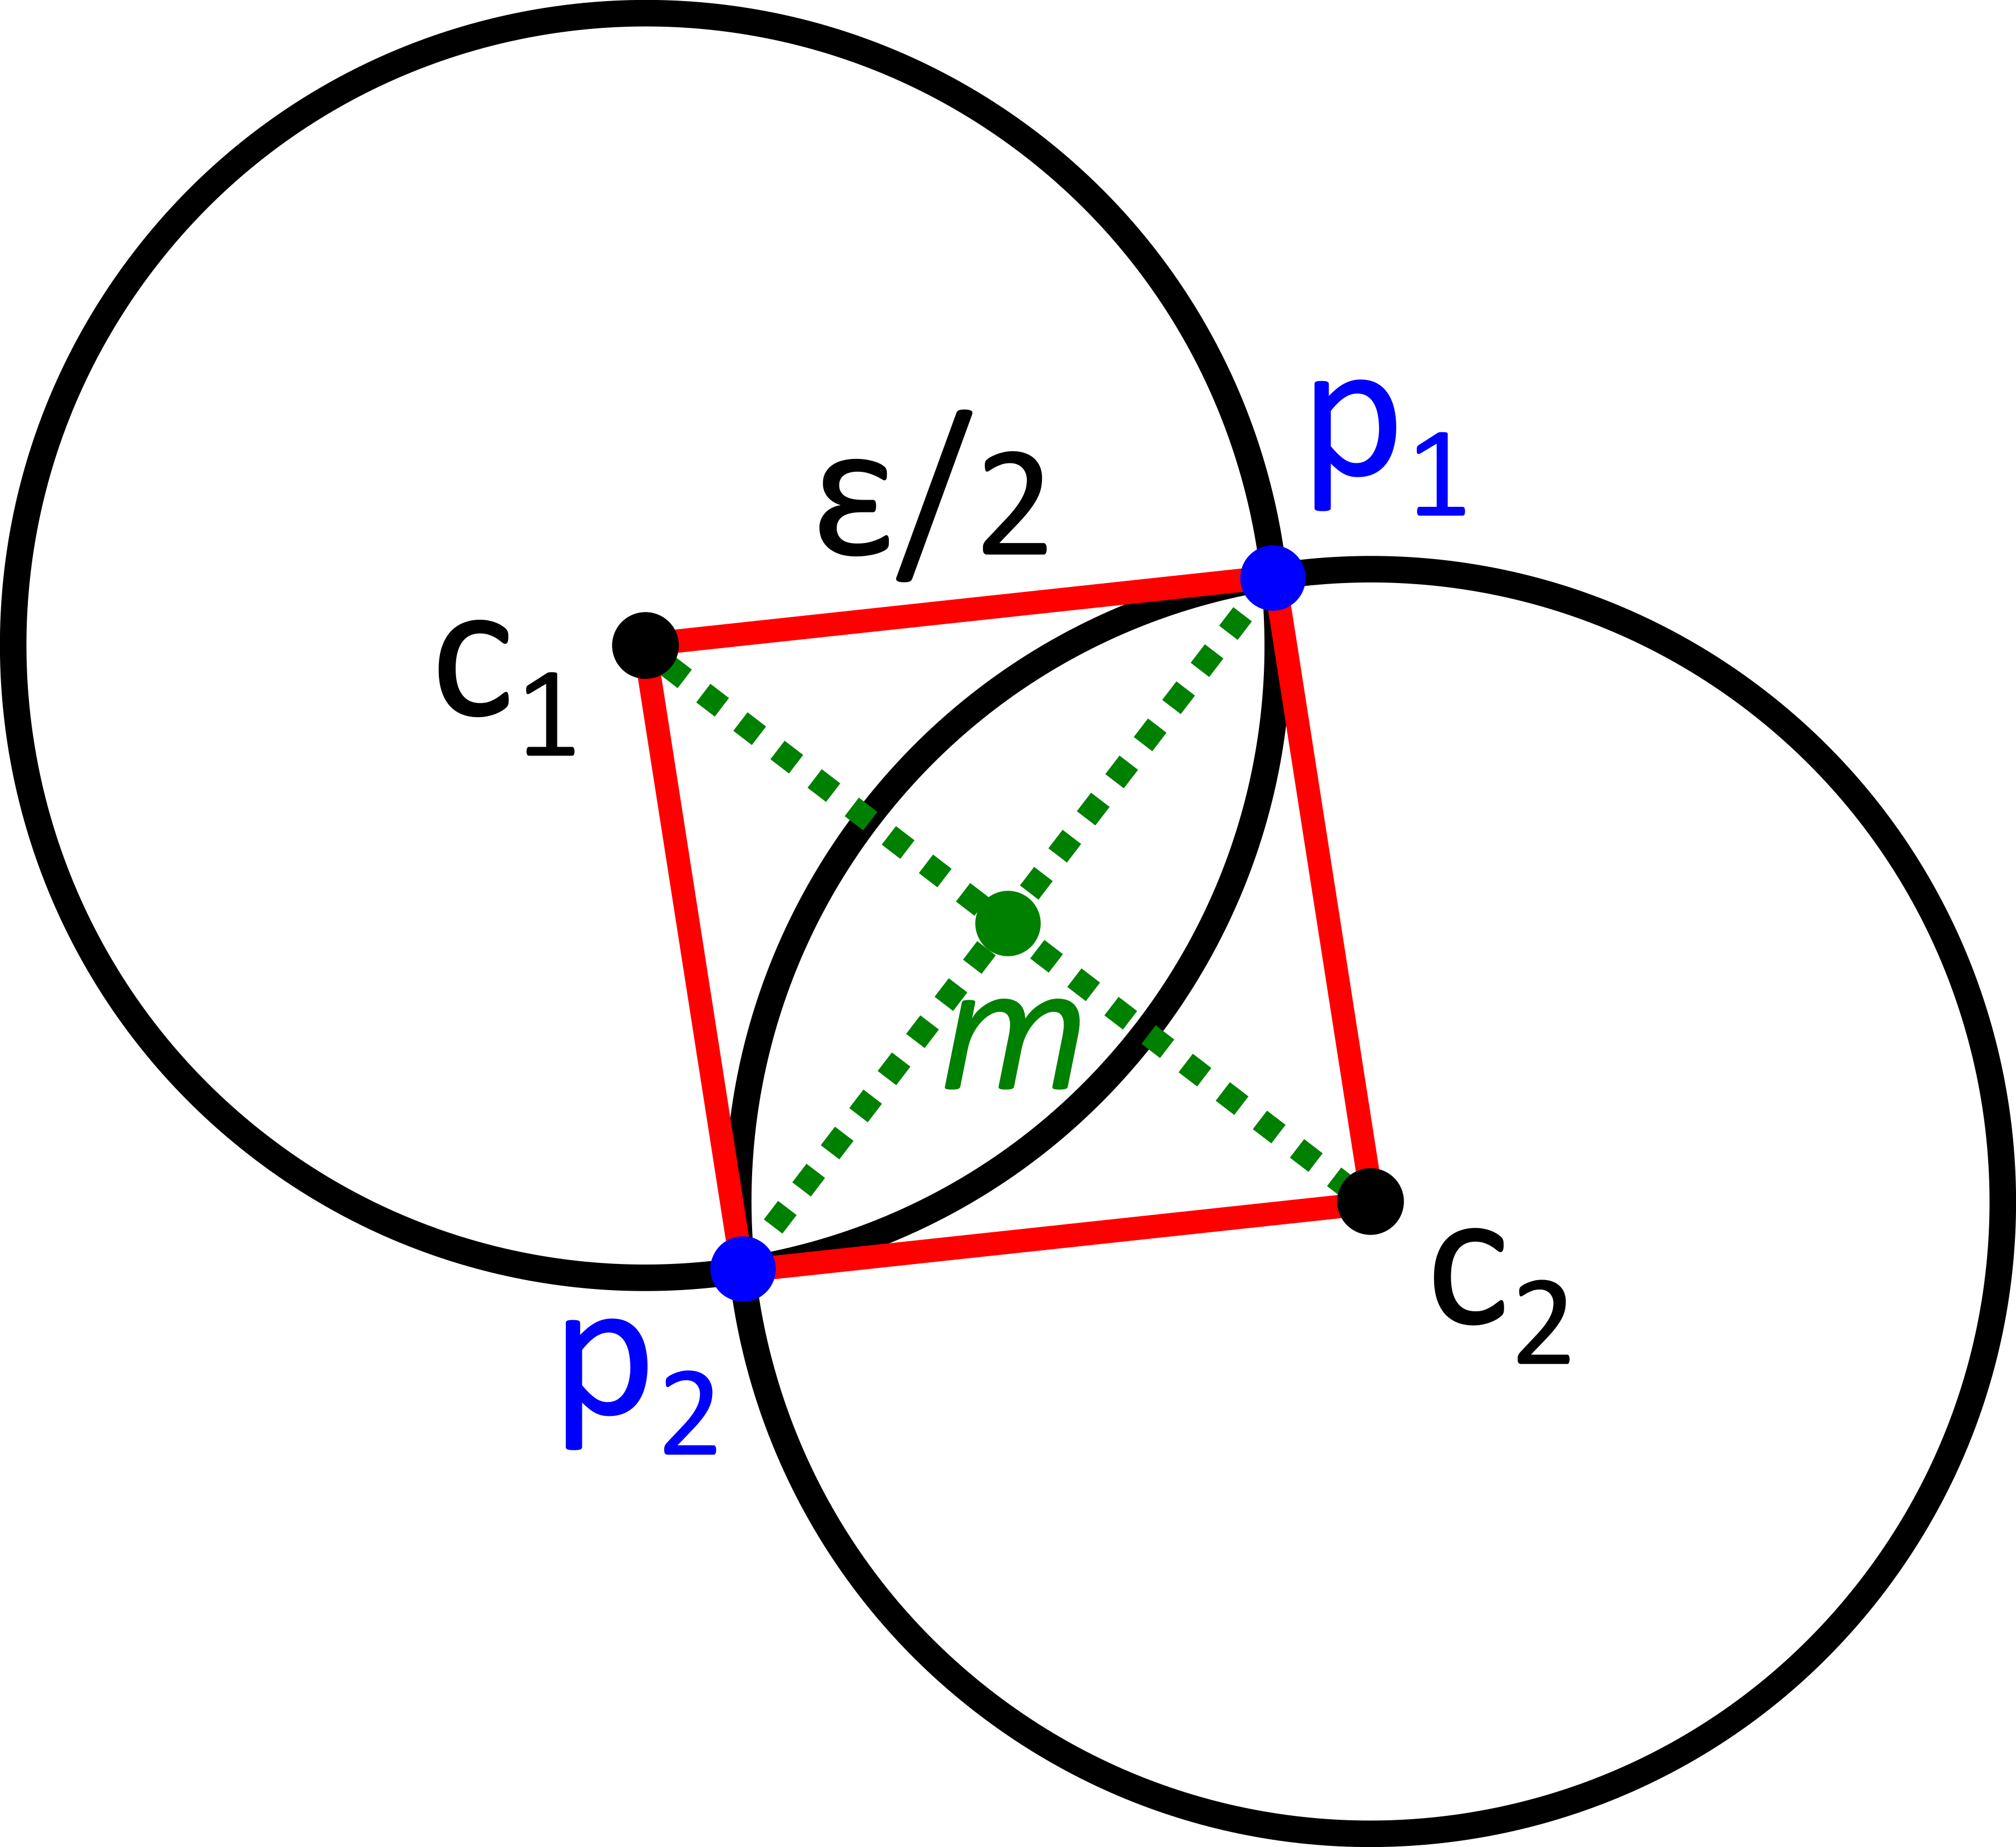
\includegraphics[width=0.7\textwidth]{images/disks_discovery.png}}
    \footnotesize{Source: Made by the author.}
    \label{fig:disks_discovery}
\end{figure}

In order to avoid running Algorithm~\ref{alg:disks} through all the points found in a time slot $t_i$, Vieira et al.
\citep{vieira} proposed a grid structure to reduce the search space for the set of points. In that approach, all points
that belong to time slot $t_i$ will be arranged into a grid with cells of size $\epsilon$. After that, we will go
through each cell $g_{i,j}$ in the grid and perform a search for points that are at most $\epsilon$ distant from each
other. That search can be restricted to the cells $g_{i - 1, j - 1} ... g_{i + 1, j + 1}$, as depicted in
\figref{fig:grid}, because all cells have $\epsilon$ as their sizes. It is important to note that the size of $\epsilon$
directly impacts in the number of cells and the number of points in each cell. For example, for a very small $\epsilon$
more cells will be created and less points will be present in each cell.  O the other hand, large $\epsilon$ will create
less but more populated cells.

Algorithm~\ref{alg:grid} shows how we will construct the grid structure for a set of points from a specific time slot
$t_i$. In order to represent a grid structure, we will use a map of indexes to a list of points, which will then be
populated as follows. For each point $p$ in the point set, we will \textit{bucketize} the longitude and the latitude of
the point (both converted to meters, using \eqnref{eq:timeslot}) by dividing them by the cell size $\epsilon$ (lines 5
and 6). Once we have the division results, we will convert them to string and concatenate them, forming a cell index
(line 8). With the cell index in hand, we only need to add the point to the corresponding cell (line 9). It is worth
noting that this proposed approach will not create empty cells, saving memory and unnecessary cell traversing time.

\begin{algorithm}[h!]
\caption{Construct Grid}
\label{alg:grid}
\begin{algorithmic}[1]
    \State $grid \gets map\{index, [...]\}$ \Comment map of cell index to list of points that belong to that cell
    \State $points \gets \Call{GetPointsOfTimeSlot}{t_i}$
    \State
    \For{each point $p$ in $points$}
        \State $xIndex \gets \floor*{\frac{p.longitudeMeters}{\epsilon}}$
        \State $yIndex \gets \floor*{\frac{p.latitudeMeters}{\epsilon}}$
        \State
        \State $index \gets \Call{ToString}{xIndex} + "\_" + \Call{ToString}{yIndex}$
        \State $grid[index].add(p)$
    \EndFor
\end{algorithmic}
\end{algorithm}

\begin{figure}[t!]
    \centering
    \caption{Cell grid for time slot $t_i$. The dark grey is the cell that is currently being processed and the light
        gray cells around are the grids that will be in the search space of the dark cell. Each small circle inside the
        grid, represents a \ac{gps} point that was collected in time slot $t_i$}
    \centerline{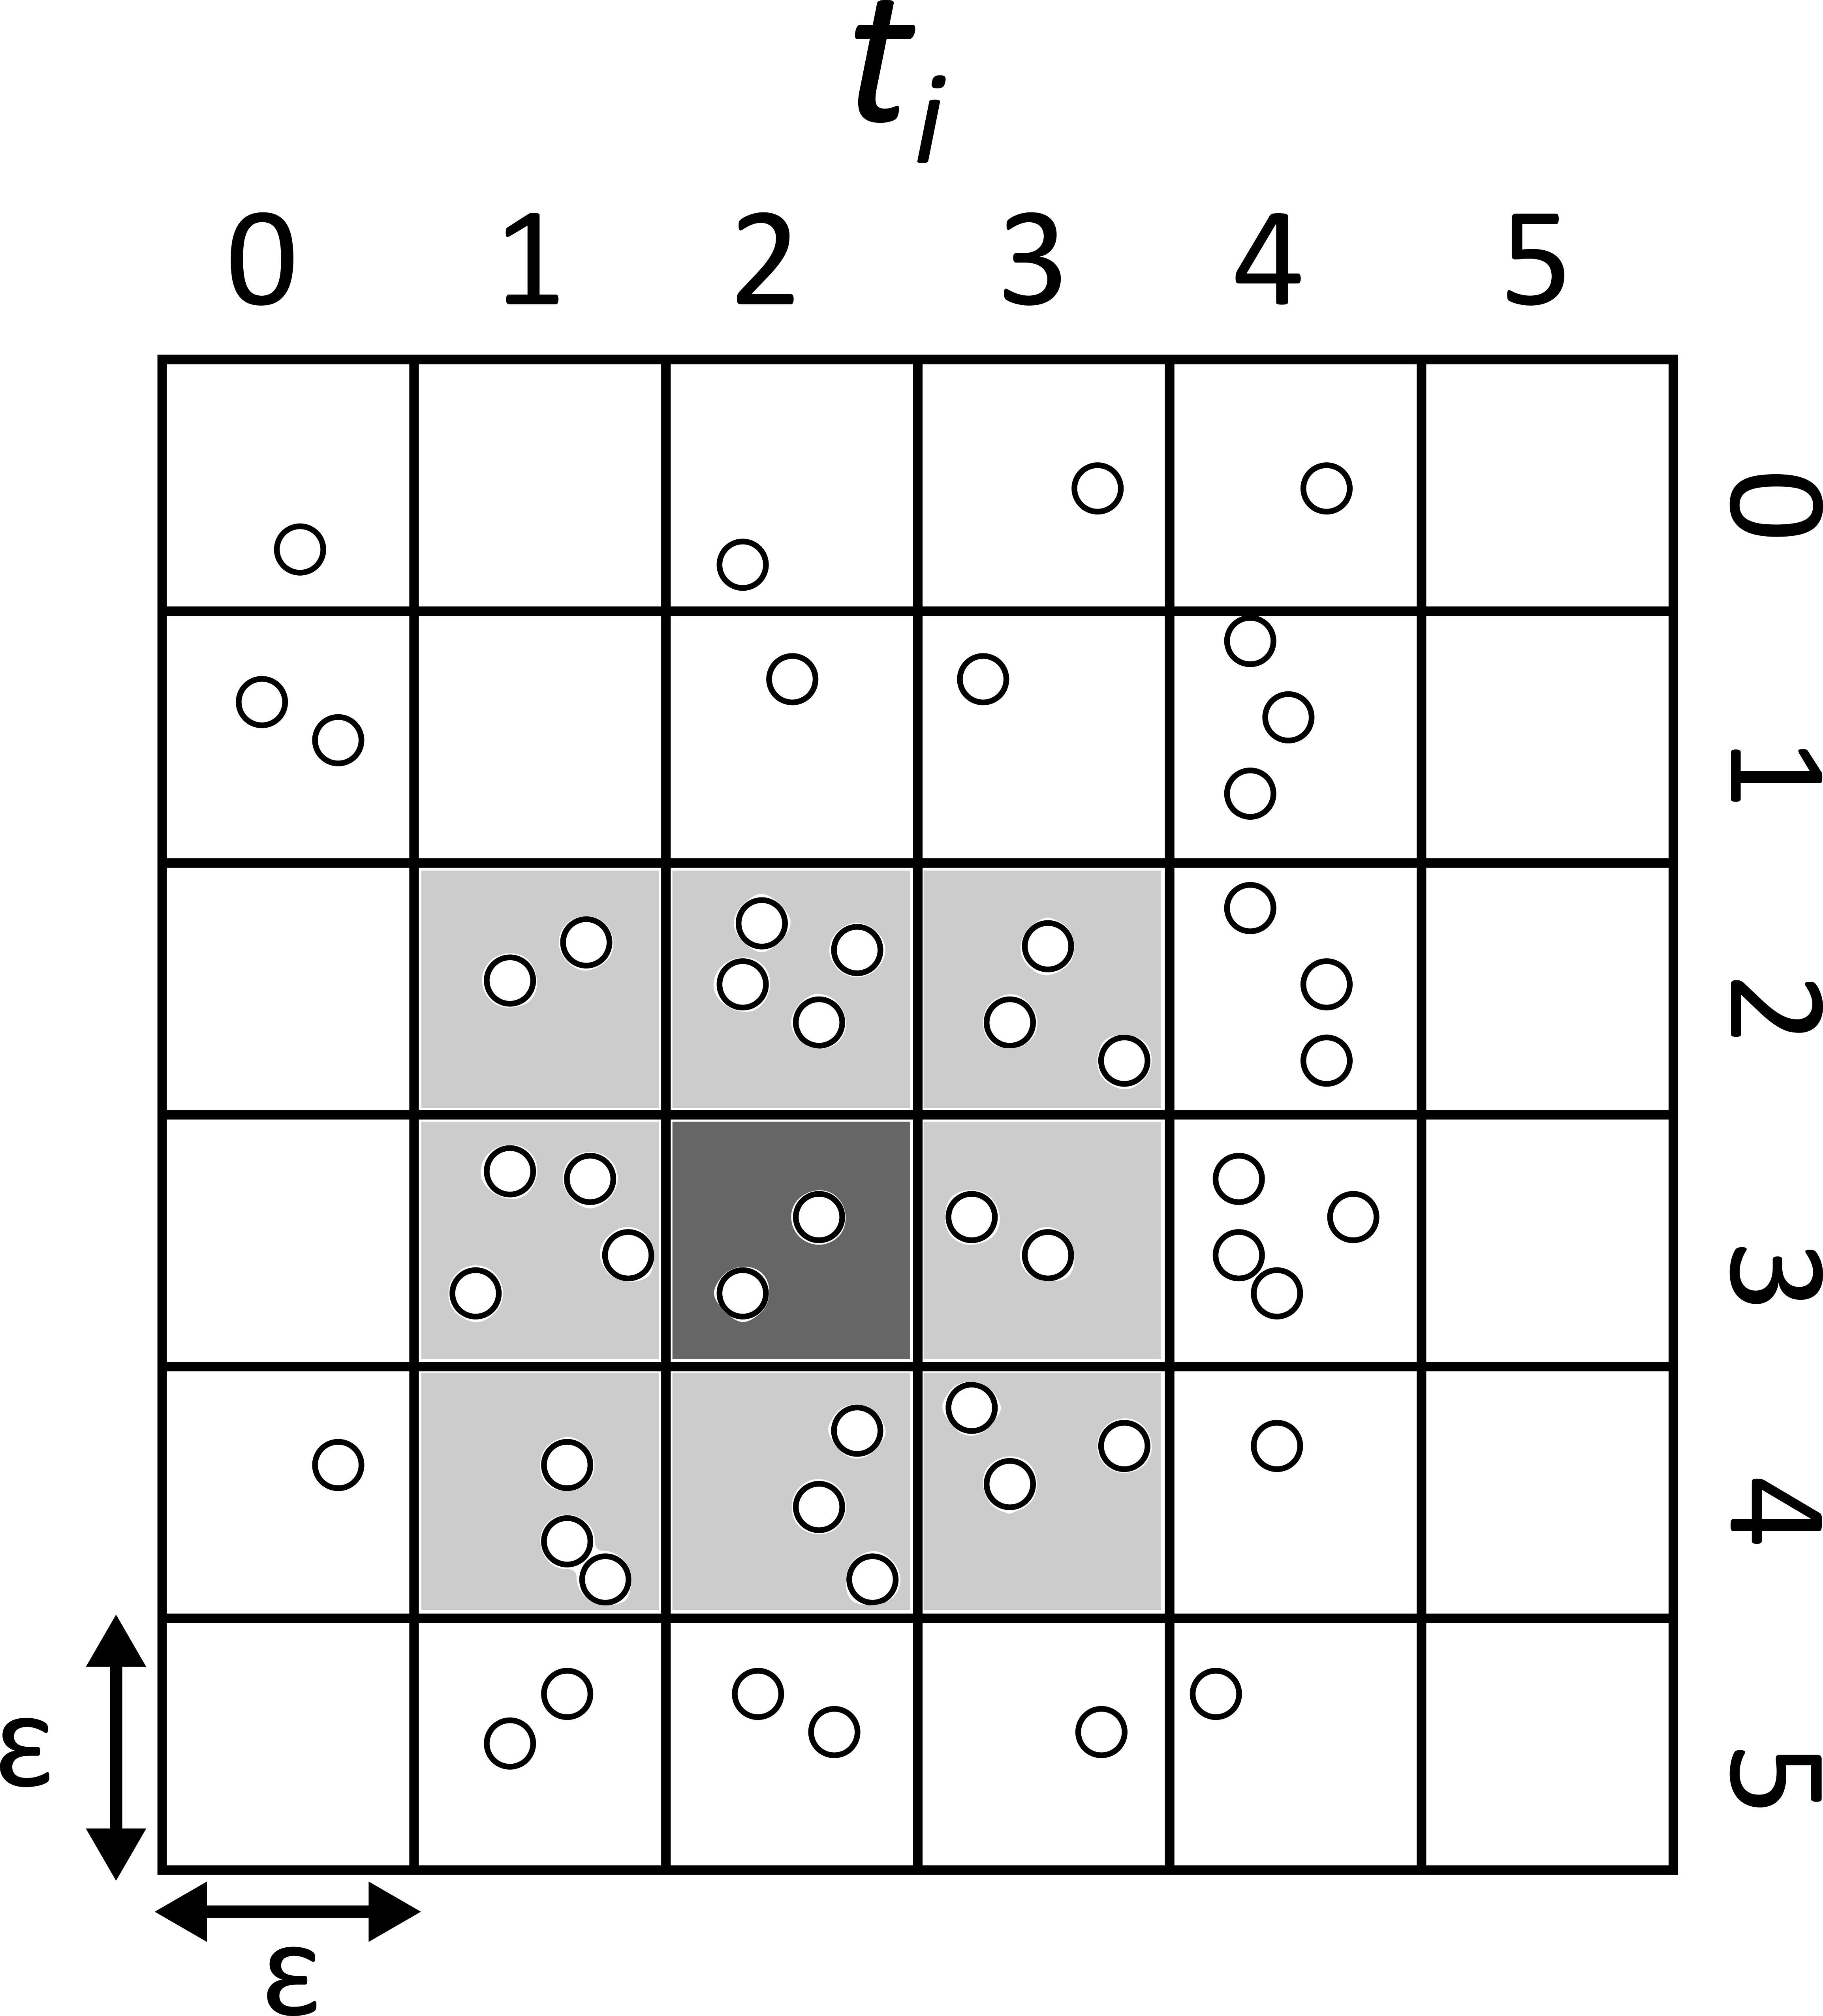
\includegraphics[width=0.7\textwidth]{images/grid.png}}
    \footnotesize{Source: Made by the author.}
    \label{fig:grid}
\end{figure}

Another important concept to keep in mind is that we are only interested in the maximum disks. Once we have found the
disks with the points that belong to them, we will check if any disk $d_i$ is a subset of another disk $d_j$. By saying
that $d_i$ is a subset of $d_j$ we mean that $d_j$ has all the points that $d_i$ has. This was identified as being a
tremendous processing bottleneck for an algorithm that aims at finding flock patterns.
